\chapter{Аппаратура и условия наблюдений в эксперименте Конус-Винд}\label{KW_description}

Рассматриваемые в работе данные получены с помощью сцинтилляционного гамма-спектрометра 
Конус, предназначенного для изучения космических гамма-всплесков, мягких гамма-репитеров и солнечных вспышек,
установленного на космическом аппарате (КА) \textit{GGS-Wind}, лаборатории NASA по изучению 
солнечно-земных связей. КА был запущен в 1994 году на сложную высокоапогейную орбиту 
с удалением до двух миллионов километров от Земли. В настоящее время КА находится 
на орбите вокруг точки либрации $L_1$ системы Земля-Солнце на расстоянии около 1.5~миллионов километров от Земли.
Подробное описание гамма-спектрометра Конус-Винд (KW) дано в работе~\citep{Aptekar_1995SSR}.

Эксперимент Конус-Винд состоит из двух одинаковых NaI(Tl) сцинтилляционных 
гамма-спектрометров (S1 и S2), расположенных на противоположных сторонах 
стабилизированного вращением КА \textit{Wind}. 
Схематический вид КА и детектора приведён на рис.~\ref{img:KW_main_view}.
Оси полей зрения детекторов 
направлены в полюса эклиптики, при этом S1 направлен на южный полюс эклиптики, 
S2 на северный. Таким образом, обеспечивается обзор всей небесной сферы. 
Каждый детектор состоит из кристалла NaI(Tl) диаметром 13~см и высотой 7.5~см, 
помещенного в алюминиевый контейнер.
Эффективная площадь одного детектора составляет $\sim 80\textrm{--}160$~см$^2$ в 
зависимости от энергии падающего фотона и угла падения.  
Для снижения энергетического порога регистрации входные окна алюминиевых 
контейнеров кристаллов выполнены из бериллия толщиной 1.5~мм. 
Кристалл просматривается фотоэлектронным 
умножителем (ФЭУ) через свинцовое стекло толщиной 19~мм, служащее для снижения фонового 
излучения от космического аппарата. Описанные параметры эксперимента дают 
возможность непрерывно производить наблюдения транзиентов, таких как гамма-всплески 
и мягкие гамма-репитеры, в условиях исключительно стабильного фона, 
без затенения части небесной сферы Землей и влияния ее радиационных поясов. 

\begin{figure}[h]
  \begin{minipage}[h]{0.5\textwidth}
    \center{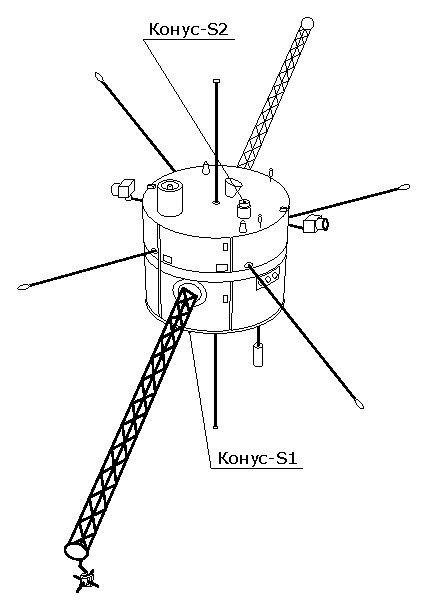
\includegraphics[height=1.0\textwidth]{wind-bw_v2} \\ а)}
  \end{minipage}
  \hfill
  \begin{minipage}[h]{0.5\textwidth}
    \center{\includegraphics[width=1.0\textwidth]{detector_ru} \\ б)}
  \end{minipage}
  \caption[Схематическое изображение КА \textit{GGS-Wind} и детектора KW.]
  {Схематическое изображение КА \textit{GGS-Wind}~(а) и детектора KW~(б).}
  \label{img:KW_main_view}  
\end{figure}

Детекторы KW работают независимо друг от друга в двух режимах наблюдений: 
фоновом и триггерном. Переход в триггерный режим происходит при статистически 
значимом превышении скорости счета над фоном $\approx 9\sigma$\footnotemark, 
где $\sigma$~--- стандартное отклонение фона, на интервале 1~с или 140~мс 
в энергетическом диапазоне 50--200~кэВ. При этом скорость счёта фона 
определяется на предшествующем интервале длиной 30~с. В фоновом режиме ведется 
непрерывная запись временной истории в трёх каналах G1 (13--50~кэВ), G2 (50--200~кэВ) 
и G3 (200--760~кэВ) с временным разрешением 2.944~с\footnotemark. В триггерном режиме запись 
временной истории ведется в тех же энергетических каналах с временным разрешением 
от 2 до 256~мс в интервале от -512~мс до 229.632~с относительно времени срабатывания 
триггера.

\footnotetext{
KW имеет три аналоговых интенсиметра с временами интегрирования 30~с, 1~с и 0.140~с. 
Триггер вырабатывается, если напряжение в интенсиметрах с масштабами 1~с или 0.140~с 
превышает напряжение в интенсиметре с временем интегрирования 30~c. 
При этом число отсчётов явно не вычисляется.
}

\footnotetext{
В некоторую часть времени, когда КА \textit{Wind} находился недалеко от Земли, 
запись велась с разрешением 1.477~с.
}

Спектральные данные представляют собой 64 спектра. Первые четыре имеют фиксированное время накопления 64~мс.
Для последующих 52-х спектров время накопления изменяется от 0.256 до 8.192~с, 
в зависимости от текущей скорости счёта в окне G2. Последние 8 спектров имеют время накопления 8.192~с. 
В результате минимальное время измерения спектров составляет 79.104~с, а максимальное~--- 491.776~с.
Измерение спектров ведётся тремя анализаторами амплитуд импульсов ФЭУ, соответствующих
двум перекрывающимся энергетическим диапазонам:  
PHA1~(13--760~кэВ), PHA2~(0.16--10~МэВ) и PHA3 (дублирует PHA1), каждый из которых 
разделён на 63 квазилогарифмических энергетических канала. 
Изменения временного разрешения по ходу записи временной истории и спектров связаны 
с существенными ограничениями на объем телеметрии, 
выделенной для эксперимента Конус (55~бит~с$^{-1}$). Результаты измерений записываются в оперативную 
память прибора. По окончании триггерного режима информация медленно переписывается 
в бортовую память, на что уходит 1--1.5~часа. На время перезаписи работа прибора 
в фоновом режиме прекращается. В это время резервирующая система продолжает измерения
скорости счета в окне G2 по каналу служебной телеметрии с разрешением 3.680~с.

\section{Функция отклика детектора}
Попадая в детектор, гамма-квант передаёт часть или всю свою энергию веществу 
сцинтиллятора, которая преобразуется в световую вспышку, регистрируемую ФЭУ. 
Заряд, собранный с анода ФЭУ, преобразуется в импульс напряжения, который усиливается и формируется для получения 
максимального отношения сигнал-шум, после чего амплитуда импульса измеряется 
аналого-цифровым преобразователем (АЦП). 

В общем виде исходный спектр излучения $f(E)$ связан с аппаратным спектром амплитуд 
импульсов $C(i)$ соотношением:
\begin{equation}\label{eq:response}
    C(i)=\int_{0}^{\infty} f(E)G(E,i) dE \mbox{ ,}
\end{equation}
где $G(E,i)$~--- функция отклика детектора, которая описывает вероятность кванту 
с энергией $E$ дать отсчёт в канал АЦП с номером $i$. На практике интегрирование 
заменяют суммированием, для KW функция отклика рассчитывается для 255 
значений энергии в диапазоне 5~кэВ--30~МэВ и 20 углов падения 
от 0$^\circ$ до~95$^\circ$ с шагом~5$^\circ$.

В общем случае невозможно получить исходный спектр $f(E)$, зная $C(i)$, из 
уравнения~\ref{eq:response}.  Эта проблема решается выбором физически обоснованной 
спектральной модели и определением её параметров подгонкой под аппаратный спектр. 
Подгонка осуществляется методом минимизации
\begin{equation}\label{eq:chisq}
    \chi^2=\sum\limits_{i=1}^n(C(i)-C_\rmn{M}(i))^2/C(i) \mbox{ ,}
\end{equation}
где $C(i)$~--- число отсчётов в канале $i$, $C_\rmn{M}(i)$~--- предсказанное моделью число отсчетов в канале, 
полученное свёрткой модели с функцией отклика (выражение~\ref{eq:response}).

Расчет матрицы отклика детектора осуществляется следующим образом.
Сначала с помощью библиотеки Geant4~\citep{GEANT4_2003NIMPA} методом Монте-Карло 
моделируются спектры потерь энергий гамма-квантов в кристалле NaI(Tl), затем на 
полученные спектры накладывается энергетическое разрешение детектора.
Подробное описание методики расчета матриц отклика детекторов KW методом Монте-Карло 
и используемых процедур восстановления фотонных спектров падающего излучения 
приведены в работе~\citep{Terekhov_1998AIPC}.

\section{Калибровка спектров}
Реальные границы энергетических диапазонов изменяются со временем в сторону 
увеличения нижнего порога энергии регистрируемых гамма-квантов, это  
связано с накоплением радиационных дефектов в детекторе под воздействием 
космических лучей и деградацией фотокатода ФЭУ. Определить реальное значение 
границ диапазонов можно благодаря наличию в спектрах фоновых линий 186~кэВ, 511~кэВ и~1460~кэВ.

Линия 186~кэВ связана с превращением изотопа $^{123}\rmn{I}$, образующегося в 
сцинтилляторе под действием космических лучей, в $^{123}\rmn{Te}$ посредством 
электронного захвата, $T_{1/2}=13$~часов. Ядро $^{123}\rmn{Te}$ образуется в 
возбужденном состоянии. Возбуждение с наибольшей вероятностью снимается излучением $\gamma$-кванта 
с энергией 159~кэВ. Заполнение вакансии на K-оболочке происходит с излучением 
рентгеновских $\rmn{K}_{\alpha}$ линий с энергиями $\approx 27$~кэВ.

Линия 511~кэВ связана с аннигиляцией позитронов после образования электрон-позитронных 
пар в материалах космического аппарата фоновыми гамма-квантами с энергиями $>1022$~кэВ.

Наиболее интенсивная линия 1460~кэВ сопровождает распад радиоактивного 
изотопа $^{40}\rmn{K}$, содержащегося в стекле, соединяющим кристалл и ФЭУ. 
Изотоп имеет два канала распада: $\beta^{-}$ в $^{40}\rmn{Ca}$ с 
вероятностью 89.3\% и электронный захват в $^{40}\rmn{Ar}$ с вероятностью 10.7\%. 
Время полураспада $T_{1/2}=1.2\times10^9$ лет. Ядро $^{40}\rmn{Ar}$ образуется в
возбужденном состоянии. Возбуждение с наибольшей вероятностью снимается 
излучением гамма-кванта с энергией 1460~кэВ.

Для автоматической калибровки спектров автором настоящей работы была 
разработана процедура поиска и аппроксимации линии 1460~кэВ в аппаратных спектрах 
KW. Калибровка PHA2 выполнялась непосредственно по положению 
линии 1460~кэВ. Положение границ PHA1 определялось по перекрытию с PHA2, 
таким образом чтобы спектр отсчётов в PHA1 наилучшим образом соответствовал спектру в PHA2 
на основании статистики $\chi^2$. Разработанный метод позволяет получать калибровки 
для большинства регистрируемых всплесков.

Изменение границ энергетического диапазона KW со временем представлено 
на рис.~\ref{img:KW_E_boundaries}. Резкие изменения границ в 1994--1996 годах 
связаны с изменением коэффициента усиления по команде с Земли. Дальнейший сдвиг 
границ диапазонов связан с деградацией детекторов. Скачкообразные изменения границ с последующей релаксацией 
к предшествующему тренду связаны потоками протонов высоких энергий, ускоренных в мощных 
солнечных вспышках класса <<X>>\ (см.~рис.~\ref{img:KW_E_boundaries_features}~a). 
Годичные изменения границ диапазонов на $\approx 3$\%, хорошо заметные в 2006--2012~гг. 
(рис.~\ref{img:KW_E_boundaries_features}~б), синхронные с вариациями температуры детекторов при движении 
КА~\textit{Wind} по орбите вокруг Солнца. Однако, изменение границ не связано напрямую 
с температурой детекторов, так как годичный максимум значений границ приходится на 
начало сентября, а минимум температуры~--- на начало июля. 

Этот эффект гораздо сильнее зависимости световыхода сцинтиллятора NaI(Tl) 
от температуры и имеет противоположное направление. Зависимость световыхода NaI(Tl) от 
температуры эффективно сдвигает линию в младшие каналы при росте температуры 
(реальные значения границ каналов увеличиваются). При этом зависимость положения 
фотопика 662~кэВ ($^{137}$Cs) от температуры составляет 
не более~$-0.6\textrm{\%}/1^{\circ}\rmn{C}$~\citep{Ianakiev_2009NIMP}.

\begin{figure}[h]
  \begin{minipage}[h]{0.5\textwidth}
    \center{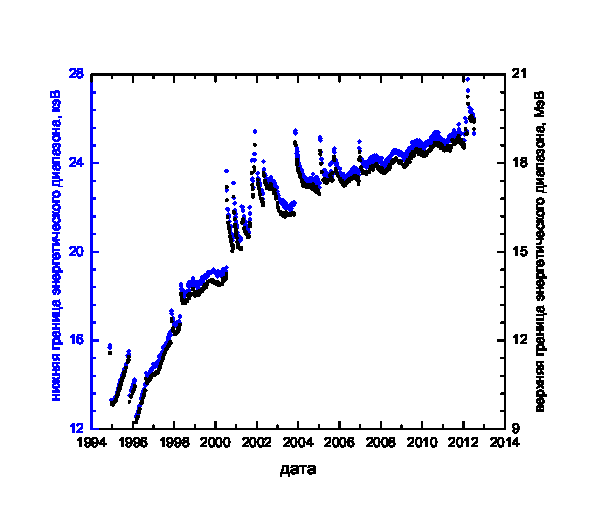
\includegraphics[width=1.0\textwidth]{gS1_calib} \\ а)}
  \end{minipage}
  \hfill
  \begin{minipage}[h]{0.5\textwidth}
    \center{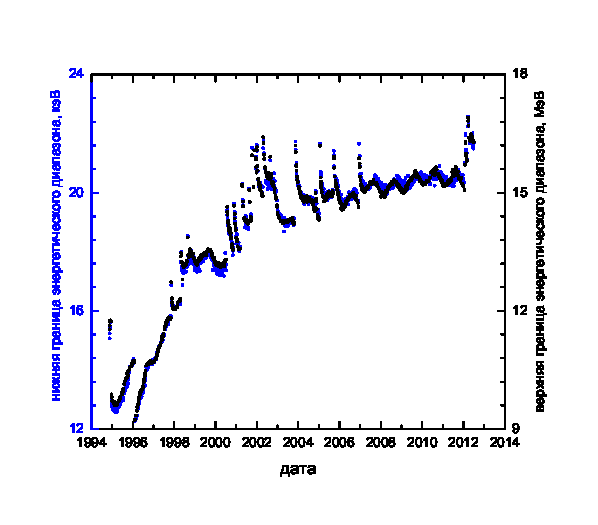
\includegraphics[width=1.0\textwidth]{gS2_calib} \\ б)}
  \end{minipage}
  \caption[Изменение со временем границ энергетического диапазона для детектора S1 и~S2.]
  {Изменение со временем границ энергетического диапазона для детектора S1~(a) и~S2~(б).}
  \label{img:KW_E_boundaries}  
\end{figure}

\begin{figure}[h]
  \begin{minipage}[h]{0.5\textwidth}
    \center{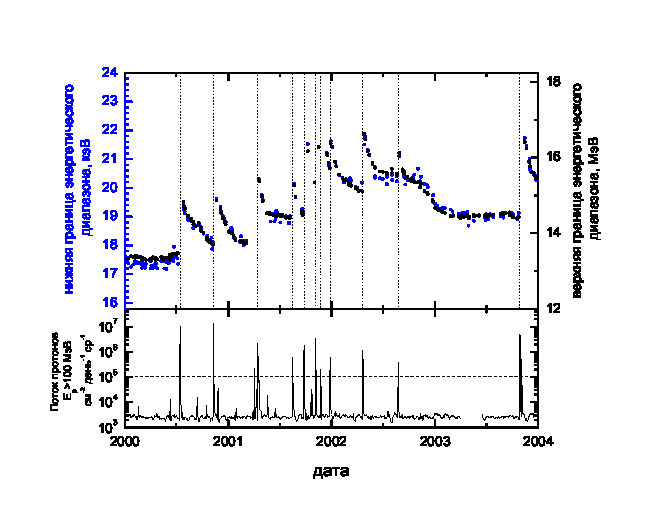
\includegraphics[width=1.0\textwidth]{gS2_protons_100MeV} \\ а)}
  \end{minipage}
  \hfill
  \begin{minipage}[h]{0.5\textwidth}
    \center{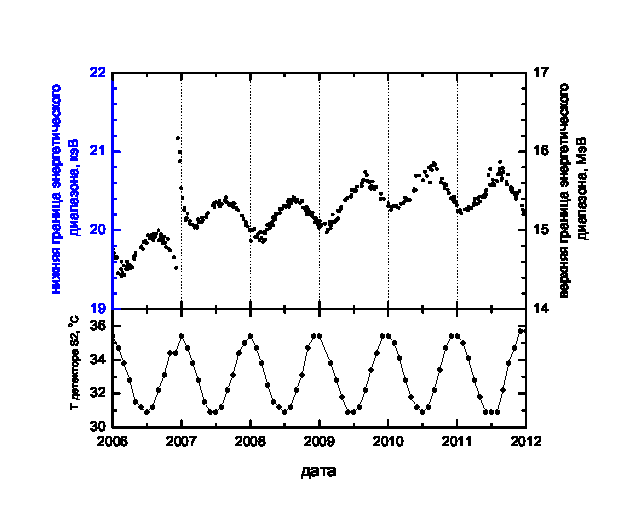
\includegraphics[width=1.0\textwidth]{gS2mE2_Temp} \\ б)}
  \end{minipage}
  \caption[Изменение со временем границ энергетического диапазона детектора S2 
  в 2000--2003~гг. и 2006--2011~гг.]
  {Изменение со временем границ энергетического диапазона детектора S2 (подробно). 
  Скачкообразные изменения границ диапазона в 2000--2003~гг. при облучении протонами с $E>100$~МэВ~(a). 
  Годичные изменения границ диапазонов в 2006--2011~гг., связанные с вариацией температуры детекторов 
  при движении КА \textit{Wind} по орбите вокруг Солнца~(б).}
  \label{img:KW_E_boundaries_features}  
\end{figure}

\section{Чувствительность детекторов}
Под чувствительностью детектора понимается минимальный интегральный поток $S$~[эрг~см$^{-2}$], 
который вызовет превышение фона в канале детектора на заданном временном интервале 
на заданное число стандартных отклонений фона. При этом искомый поток будет зависеть 
от формы спектра падающего излучения, угла падения на детектор и фоновой скорости счёта детектора.

\subsection{Фоновая скорость счёта}\label{sec:Bg_rate}
Уровень фона KW благодаря нахождению прибора в межпланетном пространстве 
может оставаться постоянным на протяжении нескольких дней в периоды низкой 
солнечной активности. При анализе временных историй большинства гамма-всплесков, 
зарегистрированных в триггерном режиме, фон аппроксимировался 
постоянным значением на интервале от $T_0 - 1000$~с до $T_0 - 250$~с, 
где $T_0$~--- время срабатывания триггера. Значительный отступ от триггерного 
времени связан с тем, что 
в случае, если всплеск имеет плавное нарастание интенсивности, 
триггер срабатывает значительно позже начала всплеска, и
значительная часть всплеска лежит вне триггерной записи. 

Для подтверждения постоянства фона на заданном интервале проверялась гипотеза о том, 
что числа отсчётов в 2.944 секундных интервалах измерения (бинах) 
имеют гауссово распределение, со средним равным среднему числу отсчётов 
в бинах $\overline{N}$ и стандартным отклонением $\sqrt{\overline{N}}$. 
Для проверки гипотезы использовался критерий Колмогорова-Смирнова с уровнем значимости 0.01~\citep{Press_1992NumRec}. 
Если гипотеза принималась, то фон считался равным вычисленному среднему. 
Если гипотеза отвергалась, то интервал сокращался на одни бин со стороны наиболее 
удалённой от $T_0$ и процедура повторялась пока не обнаруживался интервал с постоянным фоном 
или длительность интервала не достигала минимально допустимого значения 30~с. 
Для большинства всплесков длина фонового интервала равна 750~с, менее 1\% 
всплесков имеют малую длину фонового интервала 30--100~c.

Уровни фона в трех диапазонах детекторов S1 и S2 различаются, 
что связано с различием границ диапазонов в детекторах. Скорости счёта фона 
на 2015~г. и их характерные ошибки и относительное изменение по сравнению с 1994~г.
приведены в таблице~\ref{tab:bg_cnt_rate}.
В периоды повышенной солнечной активности наблюдались сильные кратковременные вариации фона. 
Изменение уровней фона со временем представлено на рис.~\ref{img:KW_bg_drift}.
Вариация фона в окне G3 хорошо отражает долговременную вариацию потока космических 
лучей в ходе 11-летнего солнечного цикла. 

\begin{table} [h]
 \centering
 \caption{Фоновая скорость чёта в детекторах KW.}
 \label{tab:bg_cnt_rate}
\scriptsize
  \begin{center}
  \begin{tabular}{c c c c c c}
  \hline
  \hline
каналы & \multicolumn{2}{c}{скорость счёта,} & характерная        & \multicolumn{2}{c}{относительное изменение, \% }\\
  & \multicolumn{2}{c}{отсч~с$^{-1}$} &   ошибка, отсч~с$^{-1}$   & \multicolumn{2}{c}{(1994--2015~гг.)}\\
       &  S1        &    S2      &                        & S1        &    S2      \\       
\hline
G1 &   950  & 1050  & 1.3 & 17 & 11\\ 
G2 &   300  & 350   & 0.7 & 52 & 45\\ 
G3 &   150  & 130   & 0.5 & 38 & 29\\ 
\hline
\end{tabular}
\end{center}
\end{table} 

\begin{figure}[h]
  \begin{minipage}[h]{0.5\textwidth}
    \center{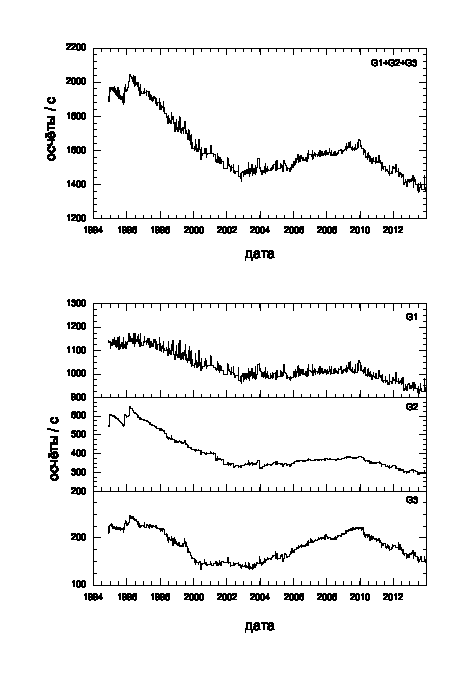
\includegraphics[width=1.0\textwidth]{gS1bg_cleaned} \\ а)}
  \end{minipage}
  \hfill
  \begin{minipage}[h]{0.5\textwidth}
    \center{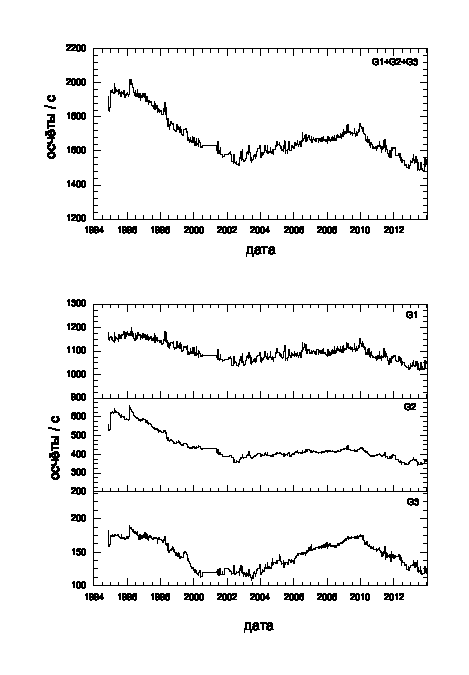
\includegraphics[width=1.0\textwidth]{gS2bg_cleaned} \\ б)}
  \end{minipage}
  \caption[Изменение со временем уровней фона детекторов S1 и~S2]
  {Изменение со временем уровней фона детекторов S1 (а) и~S2 (б). 
  Кратковременные повышения фона, связанные с потоками частиц от Солнца удалены.}
  \label{img:KW_bg_drift}  
\end{figure}

\subsection{Расчёт минимального детектируемого потока}
Зная уровень фона и форму спектра, можно вычислить интегральный поток $S$, который 
даст превышение в $k$ стандартных отклонений ($\sigma$) над фоном на временном 
интервале $\Delta T$ в одном из каналов G1, G2 или G3, или их комбинации.
Для расчёта $S$ использовались две функции, широко применяемые для моделирования 
спектров гамма-всплесков: степенной закон с экспоненциальным обрезанием (сutoff power law, CPL)
\begin{equation}\label{eq:CPL}
\frac{dN}{dE} = A \left(\frac{E}{E_n}\right)^\alpha \exp\left(-\frac{E}{E_0}\right) \mbox{ ,}
\end{equation}
где $A$~--- амплитуда [фотоны см$^{-2}$~с$^{-1}$~кэВ$^{-1}$], $\alpha$~--- показатель степени,
$E_0$~--- энергия обрезания спектра, $E_n = 100$~кэВ~--- нормировочная энергия,
и модель Банда (Band)~\citep{Band_1993ApJ}
\begin{equation}\label{eq:Band}
\frac{dN}{dE}=A \left\{
\begin{array}{lr}
\left(\frac{E}{E_n}\right)^\alpha \exp\left(-\frac{E}{E_0}\right) \mbox{, } 
&\mbox{если } E<(\alpha-\beta)E_0\\
\left(\frac{E}{E_n}\right)^\beta 
\left[(\alpha-\beta)\left(\frac{E_0}{E_n}\right)\right]^{(\alpha-\beta)} 
\exp(\beta-\alpha)  \mbox{, } &\mbox{если } E\geq(\alpha-\beta)E_0 \\
\end{array}
\right. \mbox{ ,}
\end{equation}
здесь $\beta$~--- показатель степени в области больших энергий, 
характерное значение которого $\beta = -2.5$~\citep{Goldstein_2013ApJS, Gruber_2014ApJS}. 
Энергия, на которую приходится максимум в спектре $E F_E = E^2 dN/dE$ равна $E_\rmn{p}=(\alpha+2) E_0$.

На основе заданных спектральных параметров модели и единичной нормировки $A=1$ 
вычислялся поток $F$~[эрг~см$^{-2}$~с$^{-1}$]
\begin{equation}\label{eq:flux}
F = \int_{E_\rmn{min}}^{E_\rmn{max}} E \left(\frac{dN}{dE}\right) dE \mbox{ .}
\end{equation}
Используя ту же модель, вычислялась скорость счёта от источника $R_\rmn{src}$ в 
заданном канале (G1, G2 или G3, или их комбинации) путём свёртки 
модели с трёхканальной матрицей отклика. Интегральный поток $S$, который даст 
превышение на $k$ стандартных отклонений фона $\sigma$ над фоном на интервале $\Delta T$ 
вычислялся по формуле $S = k (F/R_\rmn{src}) \sqrt{R_\rmn{bg} \Delta T}$, 
где $R_\rmn{bg}$~--- фоновая скорость счёта в канале. Формула представляет собой простой 
пересчёт порогового числа отсчётов в интегральный поток.

Зависимость интегрального потока $S$ в диапазоне 20~кэВ--10~МэВ для $k=9$ и $\Delta T=1$~c от параметров спектральных 
моделей показаны на рис.~\ref{img:KW_min_fluence}. Расчёт $S$ был проведён для уровней фона 
$R_\rmn{bg}$: 1000~отсч~с$^{-1}$, 350~отсч~с$^{-1}$ и 150~отсч~с$^{-1}$ для~G1, G2 и G3, соответственно, 
и границ каналов G1 (20--80~кэВ), G2 (80--300~кэВ) и G3~(300--1200~кэВ), 
близких к текущим значениям, и угла падения на детектор $60^{\circ}$. 

Для канала G2, на основании которого вырабатывается триггер, модель Банда даёт 
\begin{equation}\label{eq:KW_Smin}
S\mbox{(20~кэВ--10~МэВ)} \approx 1\times10^{-6}\left(\frac{k}{9}\right)
\left(\frac{R_\rmn{bg} \Delta T}{350\mbox{ отсч~с}^{-1} \cdot 1\mbox{ с}}\right)^{1/2}\mbox{ эрг~см}^{-2}\mbox{ ,}
\end{equation}
где $k$~--- значимость детектирования в $\sigma$,
для всплесков с $E_\rmn{p} \lesssim 500$~кэВ. Для всплесков, чей спектр описывается 
моделью CPL (без степенного <<хвоста>>) подобная чувствительность достигается в диапазоне $30\lesssim E_\rmn{p} \lesssim 800$~кэВ.
Для короткого триггерного интервала 140~мс и $k=9$ порог составляет ${\approx 4\times10^{-7}}$~эрг~см$^{-2}$

\begin{figure}[h]
  \begin{minipage}[h]{0.5\textwidth}
    \center{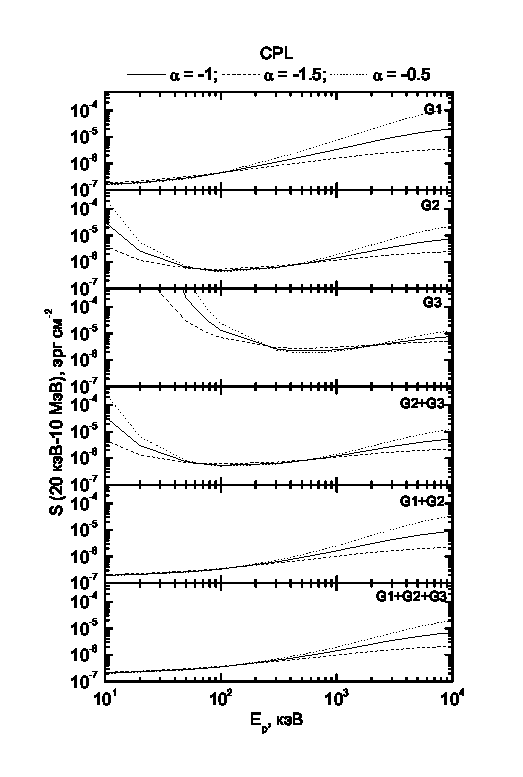
\includegraphics[width=1.0\textwidth]{gFluence_6ch_CPLru} \\ а)}
  \end{minipage}
  \hfill
  \begin{minipage}[h]{0.5\textwidth}
    \center{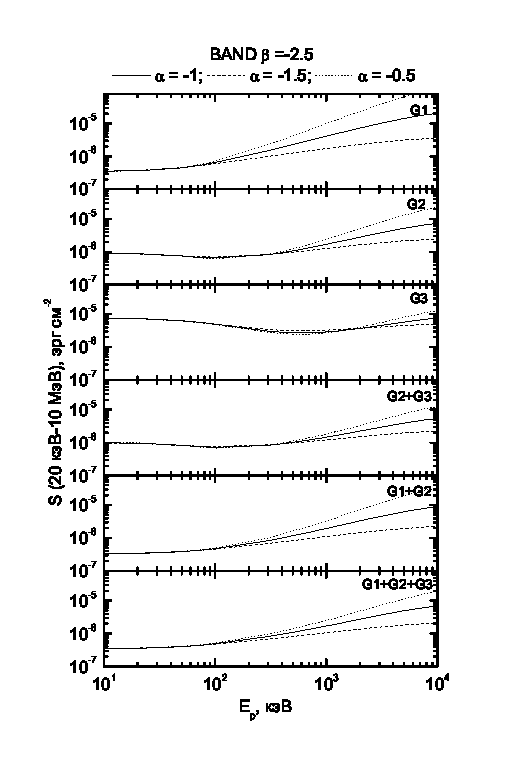
\includegraphics[width=1.0\textwidth]{gFluence_6ch_Bandru} \\ б)}
  \end{minipage}
  \caption[Минимальные регистрируемые интегральные потоки в диапазоне 20~кэВ--10~МэВ.]
  {Минимальные интегральные потоки в диапазоне 20~кэВ--10~МэВ, необходимые для детектирования 
  всплеска на уровне значимости $9\sigma$ для спектральной модели CPL с 
  показателями степеней $\alpha=-0.5$, $\alpha=-1$ и $\alpha=-1.5$~(а) 
  и~модели Band с теми же значениями $\alpha$ и $\beta=-2.5$~(б).}
  \label{img:KW_min_fluence}  
\end{figure}

\section{Заключение}
В данной главе описана методика калибровки спектрометра Конус-Винд и определения
параметров спектральных моделей. Оценена чувствительность KW. 

Получены следующие результаты:
\begin{enumerate}
\item Исследован дрейф параметров KW со временем на протяжении более 20~лет.
\item Оценен порог срабатывания триггера KW, равный $\sim 3\times10^{-7}$--$10^{-6}$~эрг~см$^{-2}$,
в зависимости от временного масштаба и параметров спектра всплеска.
\end{enumerate}

Гамма-спектрометры на основе сцинтиллятора NaI(Tl) широко применяются в астрофизических исследованиях.
Изучение изменения параметров KW на протяжении более 20~лет 
необходимо для анализа текущих данных KW и планирования будущих экспериментов. 
Благодаря положению KW в межпланетном пространстве со стабильным 
фоном излучения и практически непрерывной записи скорости счёта гамма-квантов 
(доля времени наблюдения KW, отнесённая ко всему времени работы, составляет 
примерно 95\%), полученную в диссертации методику оценки чувствительности KW 
можно использовать для оценки верхних пределов потоков гамма-излучения 
от транзиентных событий, наблюдаемых в других диапазонах длин волн, к примеру, 
от взрывов сверхновых и всплесков гравитационных волн.

Результаты расчётов, проведённых соискателем, были использованы для оценки верхних 
пределов на потоки гамма-излучения от близкой сверхновой SN~2011fe типа Ia в 
галактике M101 на расстоянии 6.4~Мпк~\citep{Margutti_2012ApJ}.

%В статье взят порог GBM цитата "We therefore conclude that there is no statistically
%significant evidence for a SN-associated burst down to the
%Fermi-GBM threshold (fluence 4*10^−8 erg cm^−2 in the 8–1000 keV band)".
%Но мин потоки Конус-Винд были важны для анализа.

\clearpage